\section{Keluarga Algoritma RC (RC5 dan RC6)}
\label{sec:rc5-rc6}

Algoritma RC dikembangkan oleh Ronald Rivest di RSA Laboratories. Nama RC sendiri
bermakna ganda: sebagian menyebutnya \textit{Rivest Cipher}, sebagian lagi
\textit{Ron's Code}. Yang dibahas pada bab ini adalah dua anggotanya, yaitu RC5 (1994)
dan RC6 (1998), yang keduanya dirancang untuk mengeksplorasi sejauh mana keamanan dapat
dicapai hanya dengan tiga operasi aritmetika yang sangat murah: XOR, penjumlahan modulo
$2^w$, dan rotasi bit \citep{rivest1994rc5,rivest1998rc6}.

\subsection{Fleksibilitas Parameter RC5}

Yang membedakan RC5 dari hampir semua \textit{block cipher} lain pada masanya adalah
bahwa ukuran blok, panjang kunci, dan jumlah putarannya semuanya dapat dipilih oleh
pengguna. Ketiga parameter itu lazim disingkat menjadi notasi
\textbf{RC5-$w$/$r$/$b$} dan diringkas pada Tabel~\ref{tab:parameter-rc5}
\citep{rivest1994rc5}.

\begin{table}[htbp]
    \centering
    \begin{tabularx}{\linewidth}{@{}l c >{\raggedright\arraybackslash}X@{}}
    \toprule
    \textbf{Parameter} & \textbf{Simbol} & \textbf{Nilai yang dibolehkan} \\
    \midrule
    Ukuran kata                    & $w$ & 16, 32, atau 64 bit (blok menjadi $2w$ bit) \\
    Jumlah putaran                 & $r$ & 0 sampai 255 \\
    Panjang kunci eksternal $K$    & $b$ & 0 sampai 255 byte, yaitu 0 sampai 2040 bit \\
    \bottomrule
    \end{tabularx}
    \caption{Parameter RC5. Blok data selalu terdiri atas dua kata, sehingga ukuran blok
    adalah $2w$ bit}
    \label{tab:parameter-rc5}
    \sumber{Munir, \textit{IF4020 Kriptografi}, ITB; Rivest, \textit{The RC5 Encryption Algorithm}.}
\end{table}

Konsekuensi penting dari parameterisasi ini perlu disadari sejak awal. Dengan $w = 32$,
RC5 beroperasi atas blok 64 bit --- sama dengan DES dan GOST. Dengan $w = 16$, bloknya
menyusut menjadi 32 bit sehingga rawan terhadap serangan berbasis paradoks ulang tahun.
Sebaliknya, $w = 64$ memberi blok 128 bit, tetapi biaya komputasinya naik. Kombinasi yang
paling banyak dipakai dalam praktik dan dalam vektor uji resmi adalah RC5-32/12/16,
yaitu blok 64 bit, 12 putaran, dan kunci 16 byte \citep{rivest1994rc5}.

\subsection{Pembentukan Kunci Putaran}

RC5 memerlukan $t = 2r + 2$ kunci putaran, masing-masing sepanjang satu kata ($w$ bit),
yang disimpan di dalam larik $S[0], S[1], \dots, S[t-1]$. Dua kunci tambahan di luar
$2r$ kunci putaran dipakai untuk penyaringan (\textit{whitening}) sebelum dan sesudah
putaran. Pembentukan larik $S$ berlangsung dalam tiga tahap.

\textbf{Tahap 1: penyalinan kunci ke larik $L$.} Kunci eksternal $K[0..b-1]$ disalin ke
larik $L$ yang beranggotakan $c$ kata, dengan

\[
c = \left\lceil \frac{b}{w/8} \right\rceil .
\]

Bila $b$ bukan kelipatan $w/8$, sisa byte pada kata terakhir diisi nol. Urutan byte di
dalam setiap kata adalah \textit{little-endian}: byte pertama menempati delapan bit
paling \emph{rendah}. Urutan ini penting, sebab implementasi yang memakai urutan
\textit{big-endian} akan menghasilkan larik $S$ yang sama sekali berbeda dan cipherteks
yang tidak dapat dipertukarkan dengan implementasi lain.

\textbf{Tahap 2: inisialisasi awal larik $S$.} Larik $S$ diisi dengan barisan
aritmetika yang dibangkitkan dari dua konstanta tetap:

\[
S[0] \leftarrow P_w, \qquad S[i] \leftarrow S[i-1] + Q_w \quad \text{untuk } i = 1, \dots, t-1 .
\]

\textbf{Tahap 3: pencampuran $L$ dan $S$.} Kedua larik dicampur sebanyak
$n = 3 \cdot \max(t, c)$ kali dengan aturan berikut, dengan $i$, $j$, $X$, dan $Y$
semuanya diinisialisasi nol:

\begin{equation}
\begin{aligned}
S[i] &\leftarrow \bigl( S[i] + X + Y \bigr) \lll 3, \qquad X \leftarrow S[i], \qquad i \leftarrow (i+1) \bmod t, \\
L[j] &\leftarrow \bigl( L[j] + X + Y \bigr) \lll (X + Y), \qquad Y \leftarrow L[j], \qquad j \leftarrow (j+1) \bmod c .
\end{aligned}
\label{eq:jadwal-kunci-rc5}
\end{equation}

Perhatikan urutan pembaruan pada Persamaan~\eqref{eq:jadwal-kunci-rc5}. Langkah $L$
memakai nilai $X$ yang \emph{sudah} diperbarui oleh langkah $S$, tetapi masih memakai
nilai $Y$ yang lama; setelah itu $Y$ baru diperbarui. Urutan ini bukan pilihan bebas:
menukarnya akan menghasilkan larik $S$ yang berbeda dan membuat implementasi tidak
kompatibel dengan vektor uji resmi. Verifikasi langkah demi langkah untuk sebuah contoh
kecil diberikan pada Contoh~\ref{ex:rc5-jadwal}.

\subsection{Konstanta \texorpdfstring{$P_w$ dan $Q_w$}{Pw dan Qw}}

Kedua konstanta pada tahap 2 tidak dipilih sembarangan, melainkan diturunkan dari dua
bilangan irasional yang terkenal:

\begin{equation}
P_w = \mathrm{Odd}\bigl( (e - 2) \cdot 2^w \bigr), \qquad
Q_w = \mathrm{Odd}\bigl( (\phi - 1) \cdot 2^w \bigr),
\label{eq:pw-qw}
\end{equation}

dengan $e = 2{,}718281828459\dots$ adalah bilangan Euler, $\phi = (1+\sqrt{5})/2 =
1{,}618033988749\dots$ adalah nisbah emas, dan $\mathrm{Odd}(x)$ menyatakan bilangan
ganjil terdekat dengan $x$. Nilai keduanya untuk ketiga ukuran kata yang didukung
diberikan pada Tabel~\ref{tab:konstanta-pw-qw}.

\begin{table}[htbp]
    \centering
    \begin{tabularx}{\linewidth}{@{}c >{\raggedright\arraybackslash}X >{\raggedright\arraybackslash}X@{}}
    \toprule
    $w$ & $P_w$ & $Q_w$ \\
    \midrule
    16 & \code{B7E1}                 & \code{9E37} \\
    32 & \code{B7E15163}             & \code{9E3779B9} \\
    64 & \code{B7E151628AED2A6B}     & \code{9E3779B97F4A7C15} \\
    \bottomrule
    \end{tabularx}
    \caption{Konstanta $P_w$ dan $Q_w$ dalam heksadesimal untuk ketiga ukuran kata RC5}
    \label{tab:konstanta-pw-qw}
    \sumber{Munir, \textit{IF4020 Kriptografi}, ITB; Rivest, \textit{The RC5 Encryption Algorithm}.}
\end{table}

Pilihan konstanta semacam ini dikenal sebagai \textit{nothing up my sleeve}: karena $e$
dan $\phi$ adalah bilangan yang maknanya sudah diketahui publik jauh sebelum RC5 lahir,
perancangnya tidak dapat menyembunyikan pintu belakang di dalam angka-angka tersebut.
Jika perancang memilih konstanta secara bebas, penyerang tidak akan pernah bisa
memastikan bahwa angka itu tidak dipilih justru untuk memudahkan serangan tertentu.

\subsection{Enkripsi dan Dekripsi}

Blok plainteks $2w$ bit dipecah menjadi dua kata, $A$ dan $B$. Enkripsi dimulai dengan
penyaringan menggunakan dua kunci putaran pertama,

\[
A \leftarrow A + S[0], \qquad B \leftarrow B + S[1],
\]

lalu dilanjutkan dengan $r$ putaran. Setiap putaran $i = 1, 2, \dots, r$ memakai dua
kunci putaran dan berbentuk

\begin{equation}
\begin{aligned}
A &\leftarrow \bigl( (A \oplus B) \lll B \bigr) + S[2i], \\
B &\leftarrow \bigl( (B \oplus A) \lll A \bigr) + S[2i+1],
\end{aligned}
\label{eq:rc5-putaran}
\end{equation}

dengan seluruh penjumlahan dilakukan modulo $2^w$ dan $\lll$ menyatakan rotasi sirkuler
ke kiri. Perhatikan bahwa jumlah pergeseran pada baris pertama adalah nilai $B$ itu
sendiri, dan pada baris kedua adalah nilai $A$ yang baru saja dihitung. Inilah yang
disebut \textbf{rotasi bergantung data} (\textit{data-dependent rotation}), dan
merupakan sumber utama nonlinearitas RC5: karena rotasi baru dapat ditentukan setelah
nilai lawan diketahui, hubungan antara bit masukan dan bit luaran berubah dari satu
blok ke blok berikutnya.

Karena rotasi bergantung data tidak linier, RC5 tidak dapat dibalik dengan mudah
seperti Feistel. Dekripsi tetap mungkin karena setiap langkah dapat dibalik satu per
satu, tetapi harus dikerjakan dalam urutan terbalik:

\[
B \leftarrow \bigl( (B - S[2i+1]) \ggg A \bigr) \oplus A, \qquad
A \leftarrow \bigl( (A - S[2i]) \ggg B \bigr) \oplus B,
\]

untuk $i = r, r-1, \dots, 1$. Setelah seluruh putaran dibalik, penyaringan awal
diperbaiki dengan mengurangkan $S[0]$ dan $S[1]$. Satu putaran RC5 digambarkan pada
Gambar~\ref{fig:putaran-rc5}.

\begin{figure}[htbp]
    \centering
    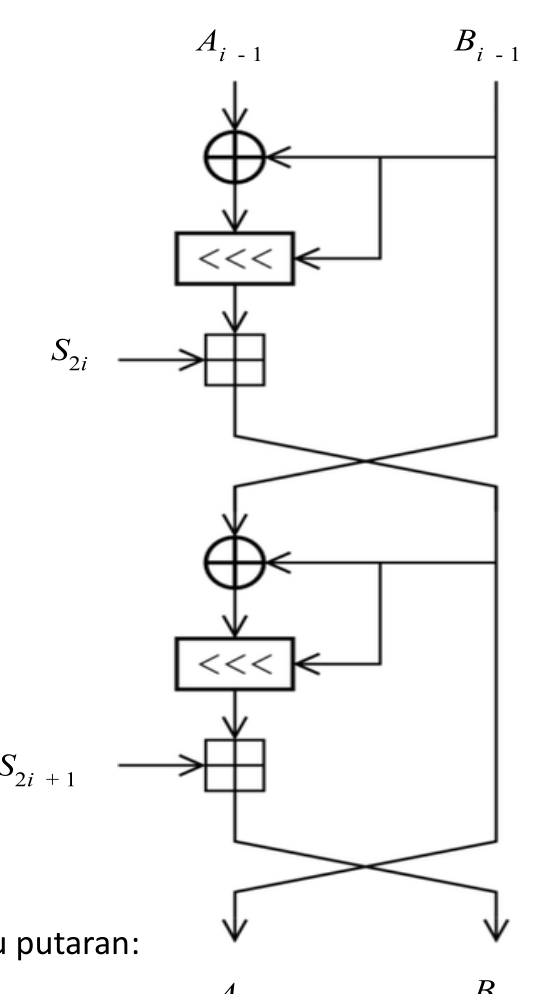
\includegraphics[width=0.8\linewidth, height=0.8\textheight, keepaspectratio]{figures/putaran-rc5.png}
    \caption{Satu putaran algoritma RC5: operasi XOR, rotasi bit ke kiri, dan penjumlahan dengan konstanta, diikuti pertukaran posisi kedua kata}
    \label{fig:putaran-rc5}
    \sumber{Munir, \textit{IF4020 Kriptografi}, ITB.}
\end{figure}

Satu catatan mengenai keamanan RC5 perlu disampaikan di sini. Karena jumlah putarannya
dapat dipilih, tidak ada satu pun nilai $r$ yang ``benar''. Rivest menyarankan $r = 12$
untuk $w = 32$ dan $r = 16$ untuk $w = 64$, tetapi rekomendasi itu dibuat pada 1994.
Serangan yang paling dikenal sejak itu menunjukkan bahwa RC5-32/12 masih bertahan,
namun dengan margin keamanan yang lebih tipis daripada perkiraan semula; varian
berputaran jauh lebih sedikit sudah dapat dibedakan dari permutasi acak. Prinsipnya
sederhana: \textit{cipher} yang parameternya bebas selalu memikul risiko bahwa pengguna
memilih parameter yang terlalu lemah.

\subsection{RC6}

RC6 dirancang oleh Rivest, Robshaw, Sidney, dan Yin pada 1998 sebagai pengembangan RC5
untuk mengikuti kompetisi AES. Perbedaan ukurannya dengan RC5 diringkas sebagai
berikut \citep{rivest1998rc6}:

\begin{itemize}
    \item Blok data bertambah menjadi 128 bit, dipegang oleh empat register $A$, $B$,
          $C$, dan $D$ yang masing-masing $w$ bit, dengan $w = 32$.
    \item Panjang kunci bervariasi dari 128 sampai 2040 bit.
    \item Jumlah kunci putaran menjadi $2r + 4$ buah, disimpan di $S[0], \dots, S[2r+3]$.
    \item Algoritma pembangkitan kunci putarannya \emph{identik} dengan RC5
          (Persamaan~\eqref{eq:jadwal-kunci-rc5}), hanya dengan $t = 2r+4$.
\end{itemize}

Operasi per putarannya pun masih XOR, penjumlahan modulo $2^w$, dan rotasi. Yang baru
adalah perkalian modulo $2^w$, yang dipakai untuk mempercepat difusi. Setiap putaran
$i = 1, \dots, r$ dihitung sebagai

\begin{equation}
\begin{aligned}
T_i &= \bigl( B_i \cdot (2B_i + 1) \bigr) \lll \lg w, \\
U_i &= \bigl( D_i \cdot (2D_i + 1) \bigr) \lll \lg w, \\
A_{i+1} &= \bigl( (A_i \oplus T_i) \lll U_i \bigr) + S[2i], \\
C_{i+1} &= \bigl( (C_i \oplus U_i) \lll T_i \bigr) + S[2i+1],
\end{aligned}
\label{eq:rc6-putaran}
\end{equation}

kemudian keempat register bergeser posisi, $(A, B, C, D) \leftarrow (B, C, D, A)$.
Setelah $r$ putaran, enkripsi ditutup dengan penyaringan $A \leftarrow A + S[2r+2]$ dan
$C \leftarrow C + S[2r+3]$.

Bentuk $x(2x+1)$ pada Persamaan~\eqref{eq:rc6-putaran} layak diperhatikan. Faktor
$2x+1$ selalu ganjil, sehingga perkalian dengannya merupakan pemetaan satu-ke-satu
modulo $2^w$; tidak ada dua nilai $x$ yang berbeda yang dapat menghasilkan luaran sama.
Hasil perkaliannya juga berderajat dua atas bit-bit $x$, sehingga jauh lebih sukar
dilinearkan daripada XOR. Kedua sifat itu dipakai oleh RC6 dengan cara yang khusus:
rotasi pada Persamaan~\eqref{eq:rc6-putaran} hanya mengambil $\lg w$ bit paling rendah
dari hasil perkalian, sehingga besarnya pergeseran ditentukan oleh seluruh bit $x$
melalui aritmetika bilangan bulat dan bukan melalui fungsi linear atas bit. Inilah
sebabnya RC6 lebih tahan terhadap kriptanalisis diferensial dan linear daripada RC5
pada jumlah putaran yang sama.

RC6 dapat dipandang sebagai dua salinan RC5 yang dijalankan secara paralel atas dua
pasang kata, dengan kedua jalur dihubungkan oleh nilai rotasi yang saling bertukar.
Cara pandang ini menjelaskan mengapa struktur keamanannya mirip RC5, sekaligus mengapa
kompleksitasnya naik: empat register berarti setiap putaran menuntut dua perkalian dan
empat rotasi, bukan dua. Pada perangkat keras berdaya rendah, biaya perkalian inilah
yang menjadi kelemahan RC6 dibandingkan Rijndael, dan hal itu ikut menjadi pertimbangan
NIST ketika memilih pemenang kompetisi AES pada Oktober 2000.
